\documentclass[12pt,a4paper]{article}
\usepackage[utf8]{inputenc}
\usepackage[T1]{fontenc}
\usepackage[english]{babel}
\usepackage{graphicx}
\usepackage[left=2.5cm,right=2.5cm,top=3cm,bottom=3cm]{geometry}
\usepackage{hyperref}
\usepackage{csquotes}
\usepackage{natbib}
\usepackage{doi}
\usepackage{amsmath}
\usepackage{booktabs}
\usepackage{listings}
\usepackage{xcolor}

\definecolor{codegray}{rgb}{0.96,0.96,0.96}
\lstset{basicstyle=\ttfamily\small,backgroundcolor=\color{codegray},frame=single,breaklines=true}

\title{Explainable Country Development Knowledge Graph\\
Trusted RDF, SPARQL, and Rule-Based Reasoning over World Bank Data}
\author{Mhd Hussam Nassif\\Group 5}
\date{19.07.2026}

\begin{document}

\maketitle

\section*{Introduction}
Country-development facts are available through trusted statistical sources, but answering questions across country metadata, indicators, classifications, and comparison rules still requires an explicit representation. A purely statistical predictor does not expose why two countries were treated as similar, whether a value came from the newest available year, or which source-specific classification was used. This project therefore transforms official World Bank data into a typed RDF knowledge graph that supports SPARQL queries and transparent inference.

The project studies three research questions. \textbf{RQ1:} Can current World Bank country metadata and indicators be transformed into a consistent RDF graph and queried correctly with SPARQL? \textbf{RQ2:} Can explicit rules and a weighted, explainable ranking produce useful country comparisons while showing their reasoning traces? \textbf{RQ3:} How accurate, complete, and consistent is the resulting system, and how do its source-grounded answers compare with closed-book answers from general-purpose language models?

The main contribution is a reproducible end-to-end system combining trusted knowledge acquisition, typed RDF, real SPARQL, symbolic rules, explainable similarity scoring, and an evaluation harness that separates model prompts from ground truth.

\section*{Background and related work}
Knowledge representation makes domain facts and relations explicit so that a system can query them and derive additional conclusions \citep{brachman2004knowledge}. Knowledge graphs represent entities as nodes and relations as edges and support integration, semantic search, question answering, and reasoning \citep{hogan2021knowledgegraphs}. RDF formalizes graph statements as subject--predicate--object triples \citep{cyganiak2014rdf}. SPARQL is the W3C query language for selecting and filtering patterns in RDF graphs \citep{harris2013sparql}.

The project also evaluates closed-book language-model answers. This comparison is motivated by research showing that language models can reproduce plausible but false or outdated statements, making explicit ground truth and repeatable scoring important \citep{lin2022truthfulqa}. The comparison in this report is deliberately small and does not claim to rank model families generally. It tests agreement with the exact World Bank snapshot; agreement on project-rule outputs is reported descriptively, not as a controlled reasoning result.

\section*{Knowledge source and representation}
The knowledge source is the official World Bank API. The Country API provides ISO codes, names, regions, income levels, lending types, capitals, and coordinates \citep{worldbankcountryapi}. The Indicators API provides time-series values \citep{worldbankindicatorsapi}. This implementation selects total population (\texttt{SP.POP.TOTL}), GDP per capita in current US dollars (\texttt{NY.GDP.PCAP.CD}), and life expectancy (\texttt{SP.DYN.LE00.IN}). Aggregate records such as ``World'' are filtered out.

The representation contains the classes \texttt{Country}, \texttt{Region}, and \texttt{IncomeLevel}. Object properties connect countries to regions and income levels. Datatype properties store names, capitals, indicator values, and years. The live run on 19 July 2026 produced 217 country entities and 3,197 RDF triples. For example:

\begin{lstlisting}
country:PAK rdf:type wbkg:Country .
country:PAK wbkg:name "Pakistan" .
country:PAK wbkg:hasRegion region:MEA .
country:PAK wbkg:hasIncomeLevel income:LMC .
country:PAK wbkg:hasCapital "Islamabad" .
country:PAK wbkg:populationTotal 255219554 .
\end{lstlisting}

This graph representation is suitable because country classification and development indicators naturally form entities, relations, and typed attributes. It also keeps the source-specific meaning visible: the current World Bank API classifies Pakistan in ``Middle East, North Africa, Afghanistan \& Pakistan'', even though general geographic descriptions often place it in South Asia.

\section*{System architecture}
Figure~\ref{fig:architecture} shows the system architecture. The acquisition layer downloads and normalizes the World Bank JSON. Country objects preserve source values and their years. RDFLib converts the objects into a typed graph and Turtle serialization. The SPARQL engine answers graph-pattern queries, while the rule components produce symbolic and scored inferences. The CLI exposes these capabilities through a live menu. A separate evaluation harness checks the representation and scores external model answers.

\begin{figure}[ht]
    \centering
    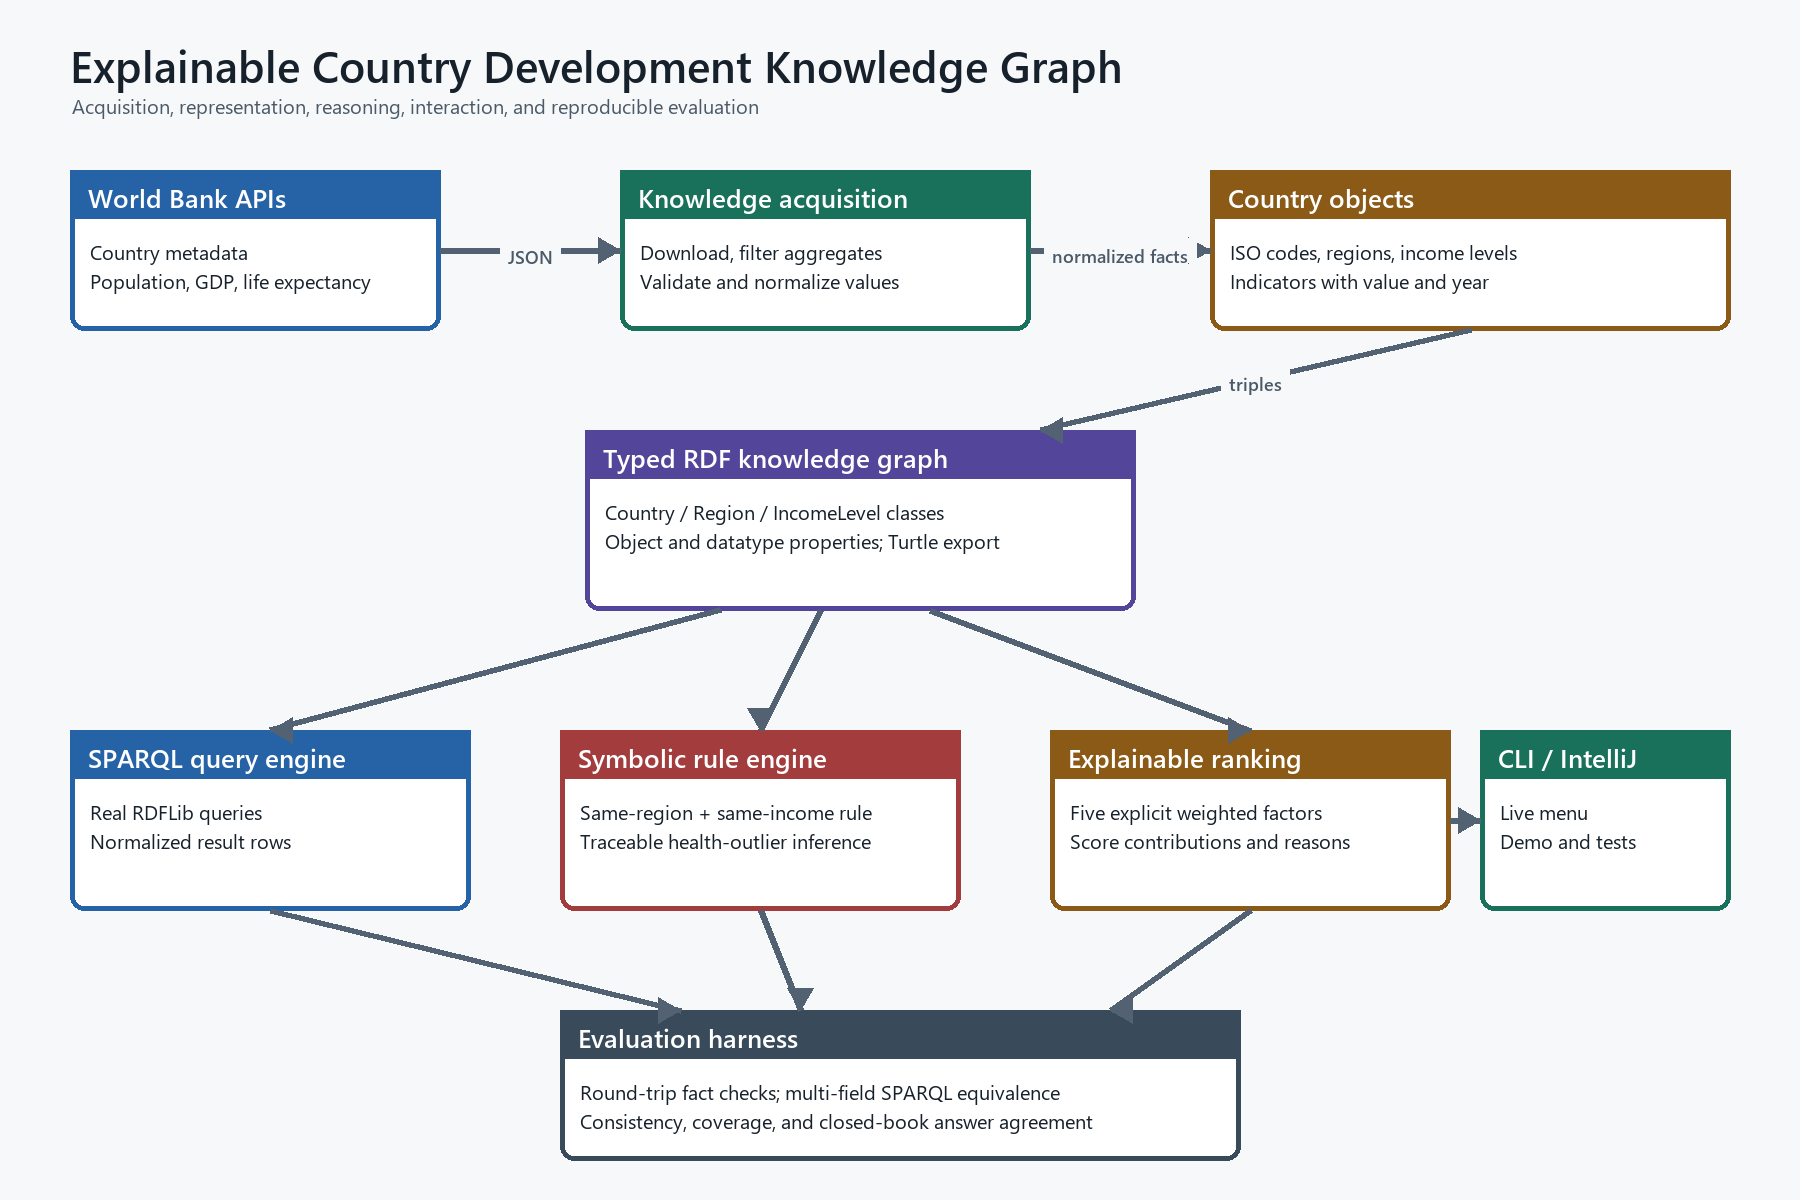
\includegraphics[width=\textwidth]{architecture_diagram.png}
    \caption{Architecture of the enhanced country-development knowledge graph.}
    \label{fig:architecture}
\end{figure}

\section{Implementation}
\subsection{Knowledge acquisition and RDF construction}
The implementation is written in Python. It requests the country endpoint and the three indicator endpoints, filters aggregate records, and joins indicator values to ISO3 country codes. RDFLib is used to create URI-identified entities, typed classes, object properties, and literal values. The resulting graph can be serialized as Turtle and parsed again by standard RDF tools.

\subsection{SPARQL querying}
The system executes real SPARQL rather than only describing a SPARQL-like interface. The following query returns Pakistan's capital and region node:

\begin{lstlisting}
PREFIX wbkg: <https://example.org/worldbank-country-kg/>
PREFIX country: <https://example.org/worldbank-country-kg/country/>
SELECT ?capital ?region WHERE {
  country:PAK wbkg:hasCapital ?capital ;
              wbkg:hasRegion ?region .
}
\end{lstlisting}

The result is \texttt{Islamabad} and \texttt{region:MEA}. The Python interface normalizes SPARQL result rows into dictionaries so that the CLI and evaluator can consume them.

\subsection{Transparent reasoning}
The original symbolic rule is retained:

\begin{lstlisting}
similar_country(X,Y) :-
    hasRegion(X,R), hasRegion(Y,R),
    hasIncomeLevel(X,I), hasIncomeLevel(Y,I),
    X \= Y.
\end{lstlisting}

The enhanced system adds an explainable similarity score:
\begin{equation}
S(X,Y)=0.30R+0.25I+0.20G+0.15L+0.10P,
\end{equation}
where $R$ and $I$ are exact region and income matches, and $G$, $L$, and $P$ are normalized closeness values for GDP per capita, life expectancy, and population. If a numeric value is missing for either country, that factor is marked unavailable and the available weights are normalized; the resulting similarity is then multiplied by evidence coverage so missing data cannot improve a country's rank. Every returned country includes the final score, available-evidence similarity, evidence coverage, each factor contribution, the available and missing factors, and human-readable reasons.

A second inference rule compares a country's life expectancy with the average of its World Bank income group. A country is inferred to be an outlier when the absolute difference is at least a configurable threshold, set to three years in the evaluation. The explanation reports the observed value, group average, direction, and difference.

\subsection{Interaction and reproducibility}
The live menu supports direct country facts, region and income queries, symbolic similarity, population thresholds, explainable similarity, health-outlier inference, and SPARQL facts. IntelliJ configurations are provided for the enhanced demo, live interaction, automated tests, and evaluation. A project-local virtual environment and pinned requirements avoid dependence on the Windows Store Python alias.

\section{Evaluation and discussion}
\subsection{Research protocol}
Evaluation has four parts. First, unit tests use synthetic countries with known expected results to test RDF typing, Turtle numeric precision, SPARQL, similarity contributions, missing-value handling, ranked scoring, and outlier traces. Second, the exported Turtle is parsed again and its RDF statements are checked against the normalized objects used by the transformation. This measures round-trip transformation fidelity, not independent accuracy of the upstream World Bank source. Third, 1,482 SPARQL-returned values for names, regions, income levels, capitals, and three indicators are compared with the Python objects, and consistency constraints detect duplicate codes, missing classifications, negative values, and invalid life-expectancy ranges. Fourth, the exploratory artifact compares seven recorded closed-book model answer sets: an older GPT-5.5 baseline, GPT-5.6 Sol, GPT-5.6 Terra, GPT-5.6 Luna, Gemini Flash, Claude Sonnet 4.5, and DeepSeek web chat. The answers were produced without project files or ground truth; raw transcripts and public run identifiers were not retained, so these results remain exploratory rather than independently auditable.

Text answers are compared after case and punctuation normalization. Unordered country lists use precision, recall, and F1; ranked answers also include positional agreement. Numeric answers use relative error with a documented tolerance. Question, ground-truth, and data-snapshot hashes prevent stale answers from being silently rescored. File separation reduces leakage risk, but raw model transcripts and decoding parameters were not retained, so the model comparison is exploratory rather than fully auditable.

\subsection{Knowledge-graph results}
\begin{table}[ht]
\centering
\small
\begin{tabular}{lr}
\toprule
Metric & Result \\
\midrule
Countries represented & 217 \\
RDF triples & 3,197 \\
RDF transformations checked & 1,699 \\
RDF transformation fidelity & 100.0\% \\
SPARQL/Python equivalence (1,482 values) & 100.0\% \\
Consistency violations & 0 \\
Population coverage & 100.0\% \\
GDP-per-capita coverage & 85.7\% \\
Life-expectancy coverage & 100.0\% \\
\bottomrule
\end{tabular}
\caption{Quantitative evaluation of the knowledge graph on 19 July 2026.}
\label{tab:kg-results}
\end{table}

The lower GDP coverage is not a representation failure: 31 represented economies had no current GDP-per-capita value in the latest API response. Missing values remain explicit rather than being guessed or imputed.

\subsection{Closed-book answer-agreement baseline}
\begin{table}[ht]
\centering
\small
\begin{tabular}{llrrrr}
\toprule
Model / tool & Provider & Status & Overall & Retrieval & Project-rule \\
\midrule
GPT-5.5 older baseline & OpenAI & Recorded & 49.0\% & 66.9\% & 1.3\% \\
GPT-5.6 Sol & OpenAI & Recorded & 42.6\% & 58.5\% & 0.0\% \\
GPT-5.6 Terra & OpenAI & Recorded & 39.8\% & 54.7\% & 0.0\% \\
GPT-5.6 Luna & OpenAI & Recorded & 36.9\% & 50.8\% & 0.0\% \\
Gemini Flash (web) & Google & Recorded & 54.8\% & 75.3\% & 0.0\% \\
Claude Sonnet 4.5 (web) & Anthropic & Recorded & 45.9\% & 63.0\% & 0.4\% \\
DeepSeek (web) & DeepSeek & Recorded & 38.0\% & 52.3\% & 0.0\% \\
\bottomrule
\end{tabular}
\caption{Closed-book answer agreement against the frozen graph. Each recorded row answered the same 11 benchmark questions.}
\label{tab:model-results}
\end{table}

All seven model runs correctly returned Islamabad and ``Lower middle income'', while all used ``South Asia'' instead of the source-specific current World Bank label ``Middle East, North Africa, Afghanistan \& Pakistan''. Gemini Flash achieved the highest overall agreement in this small run (54.8\%) and the highest retrieval agreement (75.3\%). The older GPT-5.5 baseline was second overall at 49.0\%, followed by Claude Sonnet 4.5 at 45.9\%. Several models returned population and GDP values that were plausible but different from the frozen World Bank snapshot. Agreement on project-rule questions was at most 1.3\%; this must not be interpreted as a reasoning failure because the closed-book models were not given the frozen triples needed to execute those rules.

The comparison has limitations. Eleven questions are too few for general claims, raw transcripts were not retained, each model was tested only once, and a closed-book protocol favors a system with live source access. The comparison is therefore evidence about answer agreement on this task and snapshot only. A fair reasoning follow-up should give every system the same frozen evidence packet and complete rules, use repeated runs, and report confidence intervals.

\section*{Conclusion and future work}
The enhanced project transforms trusted World Bank data into a typed RDF knowledge graph, supports real SPARQL queries, and derives explainable country-comparison and health-outlier inferences. Automated evaluation found 100\% round-trip fidelity across 1,699 checked RDF transformations, full equivalence across 1,482 SPARQL-returned values, and no tested consistency violations. The closed-book comparison illustrated where generic model variants can return common geographic categories or values that differ from the current source-specific snapshot.

Future work could add more indicators, SHACL constraints, temporal RDF statements, a web interface, and repeated cross-vendor model evaluation with retained transcripts and confidence intervals.

\bibliographystyle{plainnat}
\bibliography{literature.bib}

\vspace{0.5cm}
\hrule
\vspace{0.3em}
\hrule
\vspace{0.5em}
\begin{center}
\textbf{Source code:} \url{https://github.com/hussamn2010/worldbank-country-knowledge-graph}
\end{center}

\end{document}
